\documentclass[11pt,a4paper]{ltjsarticle}

\usepackage[top=15mm,bottom=15mm,left=15mm,right=15mm]{geometry}
\usepackage{amsmath,amssymb}
\usepackage{pdfpages}
\usepackage{bm}
\usepackage{graphicx}
\usepackage{ascmac}
\usepackage{float}
\usepackage{url}
\usepackage[hidelinks]{hyperref}
\usepackage{etoolbox}

\begin{document}
\begin{titlepage}
    \centering
    \vspace*{20mm}
    
    % 所属・講義カテゴリなど
    {\large\textgt{令和8年度 講義レポート}}\\
    \vspace{15mm}
    
    % メインタイトル（必要に応じて改行してください）
    {\huge\bfseries 画像情報処理 レポート}\\
    \vspace{5mm}
    % サブタイトル
    {\Large\textgt{-- ヒストグラムを用いたコントラスト補正と各種平滑化フィルタの特性評価 --}}\\
    
    \vspace{55mm}
    
    % 提出者情報（左寄せ・揃え）
    \begin{flushleft}
    \large
    \hspace{25mm} % 全体を少し右に寄せてバランスを取る
\begin{tabular}{rl}
        {\bfseries 科目名：} & 画像情報処理 \\ \rule{0pt}{4mm}
        {\bfseries 提出日：} & \today \\ \rule{0pt}{4mm}
        {\bfseries 所属：}   & 中部大学 工学部 情報工学科 \\ \rule{0pt}{4mm}
        {\bfseries 学籍番号：} & EP24064 \\ \rule{0pt}{4mm}
        {\bfseries 氏名：}   & 座光寺 陸 \\
    \end{tabular}
    \end{flushleft}
    
    \vfill
\end{titlepage}
\newpage

  \section{課題1}
   \subsection{実験内容}
    画質の調整(線形変換)について，プログラムのD\_max，D\_minの値を変更すると以下の画像(図\ref{fig:woman-g2})がどのように変化するか確認する．
    また，ガンマ補正についても同様にガンマ値を変更すると元画像(図\ref{fig:woman-g})がどのように変化するか確認する．
    \begin{figure}[H]
    \centering
    % 上段
    \begin{minipage}{0.45\textwidth}
        \centering
        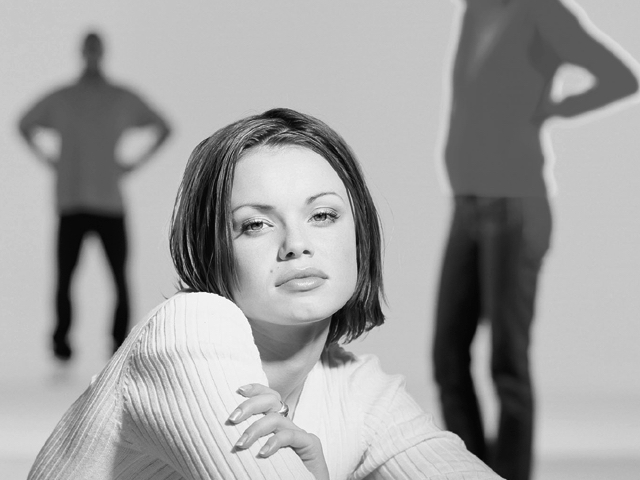
\includegraphics[width=\linewidth]{01_image/woman-g.jpg}
        \caption{元のグレースケール画像}
        \label{fig:woman-g}
    \end{minipage}
    \hfill
    \begin{minipage}{0.45\textwidth}
        \centering
        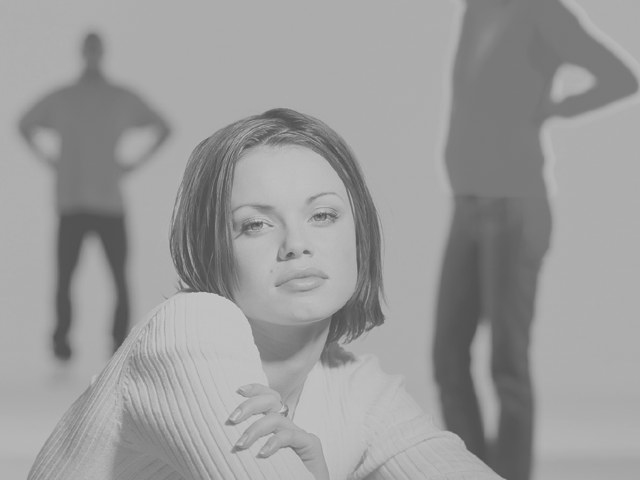
\includegraphics[width=\linewidth]{01_image/woman-g2.jpg}
        \caption{コントラストを低くしたグレースケール画像}
        \label{fig:woman-g2}
    \end{minipage}
   \end{figure}
   \subsection{線形変換の結果}
     元の画像(図\ref{fig:woman-g2})に対して(D\_max,D\_min)を変更した結果を比較する．(0,255)での線形変換後の画像を図\ref{fig:sen_defa}に，(100,255)での画像を図\ref{fig:sen_hi}に，(0,150)での画像を図\ref{fig:sen_low}に示す．
     また，各画像の画素値の分布を示す濃淡ヒストグラムについて，図\ref{fig:woman-g2}に対するものを図\ref{fig:woman-g2_hist}に，図\ref{fig:sen_defa}に対するものを図\ref{fig:sen_defa_hist}に，図\ref{fig:sen_hi}に対するものを図\ref{fig:sen_hi_hist}に，図\ref{fig:sen_low}に対するものを図\ref{fig:sen_low_hist}に併せて示す．
     \begin{figure}[H]
      \centering
      % 上段
      \begin{minipage}{0.45\textwidth}
        \centering
        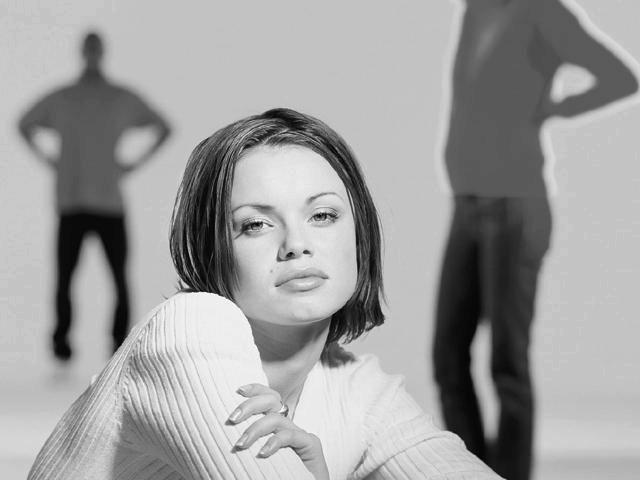
\includegraphics[width=\linewidth]{01_image/output_defa.jpg}
        \caption{(0,255)での線形変換後の画像}
        \label{fig:sen_defa}
      \end{minipage}
      \hfill
      \begin{minipage}{0.45\textwidth}
        \centering
        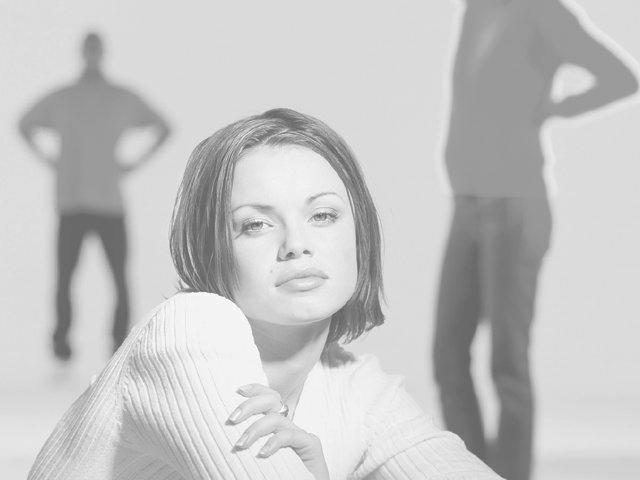
\includegraphics[width=\linewidth]{01_image/output_hi.jpg}
        \caption{(100,255)での線形変換後の画像}
        \label{fig:sen_hi}
      \end{minipage}
      \vspace{0.5cm}
      \par
    % 下段
      \begin{minipage}{0.45\textwidth}
        \centering 
        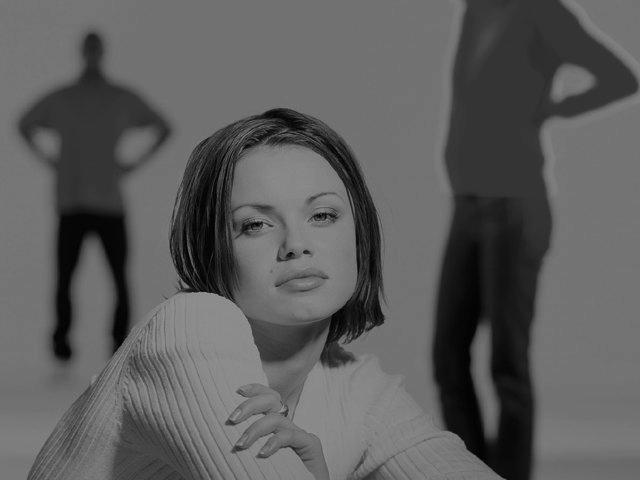
\includegraphics[width=\linewidth]{01_image/output_low.jpg}
        \caption{(0,150)での線形変換後の画像} 
        \label{fig:sen_low}
      \end{minipage}%
      \hfill
      \begin{minipage}{0.45\textwidth}
      \end{minipage}
     \end{figure}
     \begin{figure}[H]
      \centering
      % 上段
      \begin{minipage}{0.45\textwidth}
        \centering
        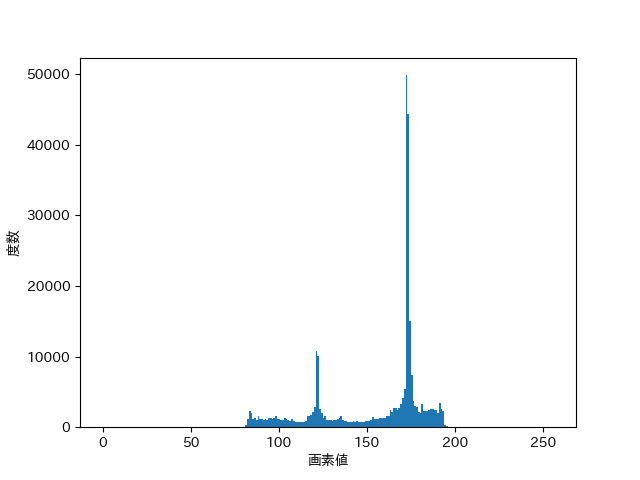
\includegraphics[width=\linewidth]{01_hist/woman_g2_hist.png}
        \caption{図\ref{fig:woman-g2}の濃淡ヒストグラム}
        \label{fig:woman-g2_hist}
      \end{minipage}
      \hfill
      \begin{minipage}{0.45\textwidth}
        \centering
        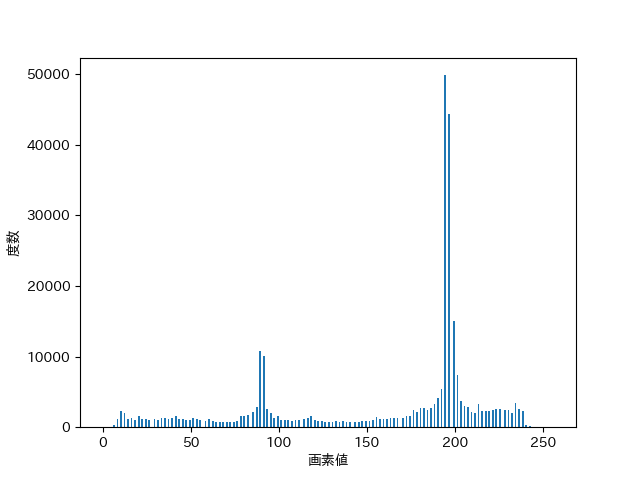
\includegraphics[width=\linewidth]{01_hist/senkei_defa_hist.png}
        \caption{図\ref{fig:sen_defa}の濃淡ヒストグラム}
        \label{fig:sen_defa_hist}
      \end{minipage}
      \vspace{0.5cm}
      \par
      \centering
      % 上段
      \begin{minipage}{0.45\textwidth}
        \centering
        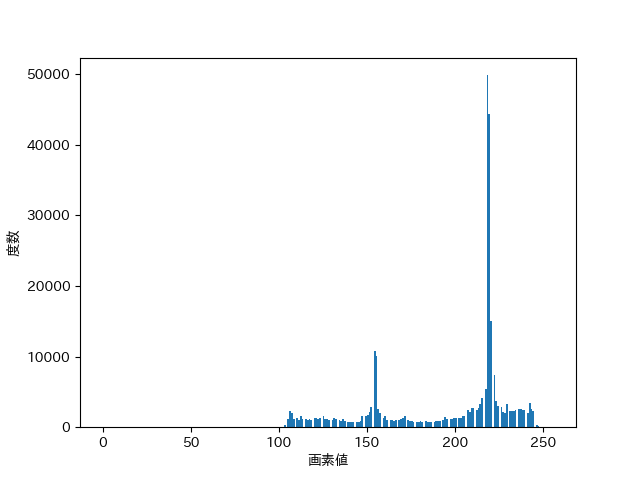
\includegraphics[width=\linewidth]{01_hist/senkei_hi_hist.png}
        \caption{図\ref{fig:sen_hi}の濃淡ヒストグラム}
        \label{fig:sen_hi_hist}
      \end{minipage}
      \hfill
      \begin{minipage}{0.45\textwidth}
        \centering
          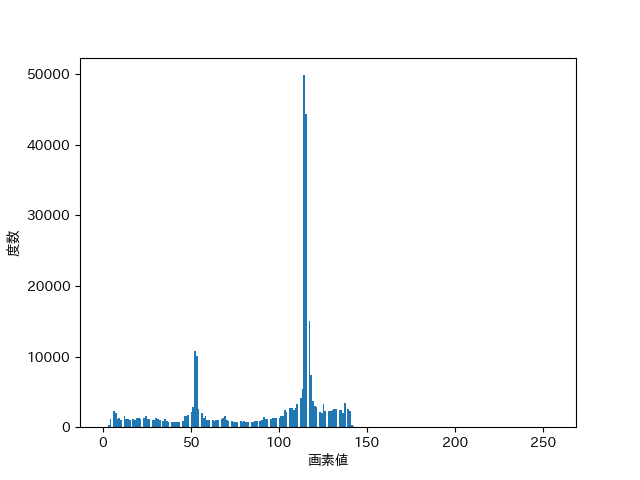
\includegraphics[width=\linewidth]{01_hist/senkei_low_hist.png}
          \caption{図\ref{fig:sen_low}の濃淡ヒストグラム}
          \label{fig:sen_low_hist}
      \end{minipage}
    \end{figure}
   \subsection{ガンマ補正の結果}
    元の画像(図\ref{fig:woman-g})に対してガンマ値$\gamma$を変更してガンマ補正を行った結果を比較する．
    $\gamma=5.0$の際の画像を図\ref{fig:gamma_defa}に，$\gamma=1.5$の際の画像を図\ref{fig:gamma_hi}に，$\gamma=0.2$の際の画像を図\ref{fig:gamma_low}に示す．
    また，図\ref{fig:woman-g}に対する濃淡ヒストグラムを図\ref{fig:woman-g-hist}に，それぞれの結果に対応する濃淡ヒストグラムを図\ref{fig:gamma_defa_hist}から図\ref{fig:gamma_low_hist}に示す．
      \begin{figure}[H]
      \centering
      % 上段
      \begin{minipage}{0.45\textwidth}
        \centering
        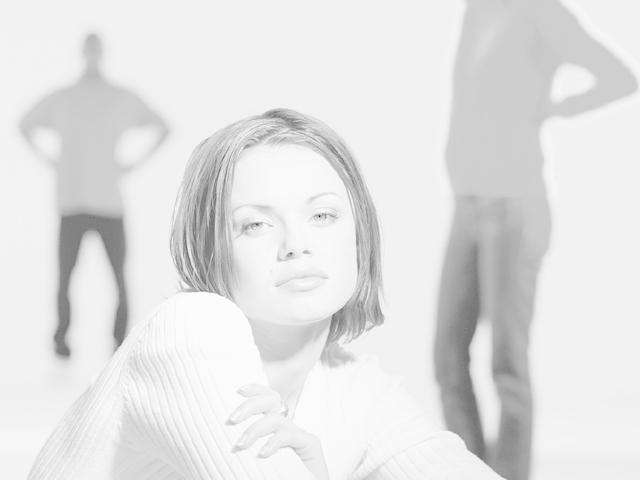
\includegraphics[width=\linewidth]{01_image/gamma_defa.jpg}
        \caption{$\gamma=5.0$のガンマ補正後の画像}
        \label{fig:gamma_defa}
      \end{minipage}
      \hfill
      \begin{minipage}{0.45\textwidth}
        \centering
        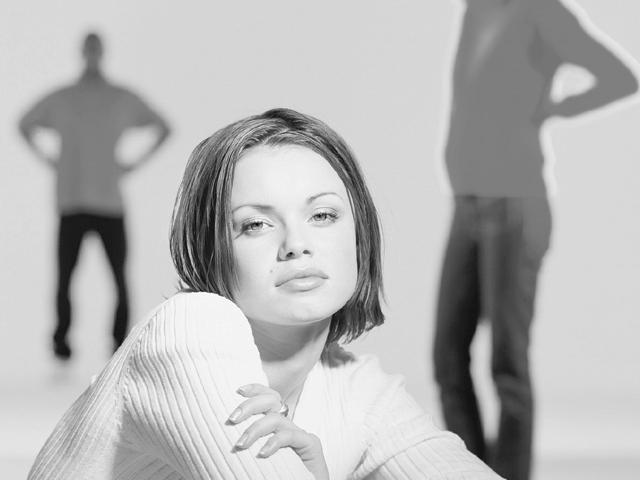
\includegraphics[width=\linewidth]{01_image/gamma_hi.jpg}
        \caption{$\gamma=1.5$のガンマ補正後の画像}
        \label{fig:gamma_hi}
      \end{minipage}
      \vspace{0.5cm}
      \par
    % 下段
      \begin{minipage}{0.45\textwidth}
        \centering 
        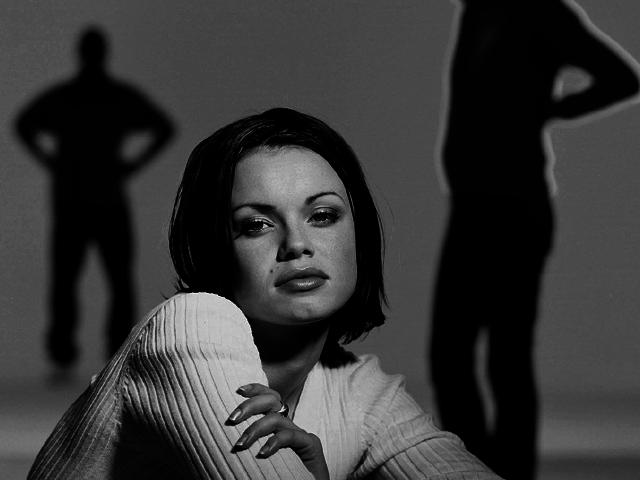
\includegraphics[width=\linewidth]{01_image/gamma_low.jpg}
        \caption{$\gamma=0.2$のガンマ補正後の画像} 
        \label{fig:gamma_low}
      \end{minipage}%
      \hfill
      \begin{minipage}{0.45\textwidth}
      \end{minipage}
     \end{figure}
           \begin{figure}[H]
      \centering
      % 上段
      \begin{minipage}{0.45\textwidth}
        \centering
        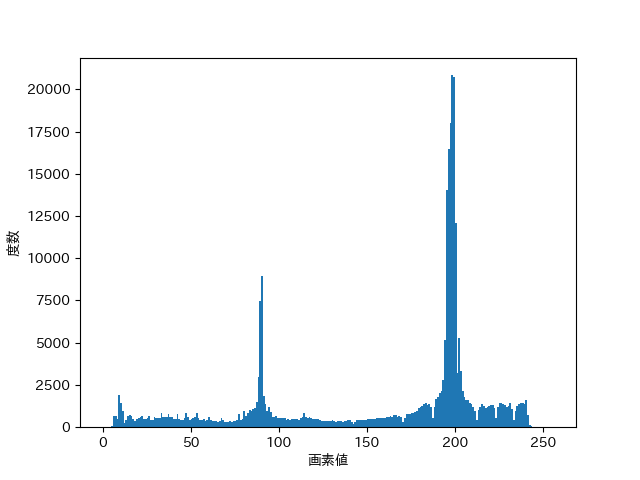
\includegraphics[width=\linewidth]{01_hist/woman_g_hist.png}
        \caption{図\ref{fig:woman-g}の濃淡ヒストグラム}
        \label{fig:woman-g-hist}
      \end{minipage}
      \hfill
      \begin{minipage}{0.45\textwidth}
        \centering
        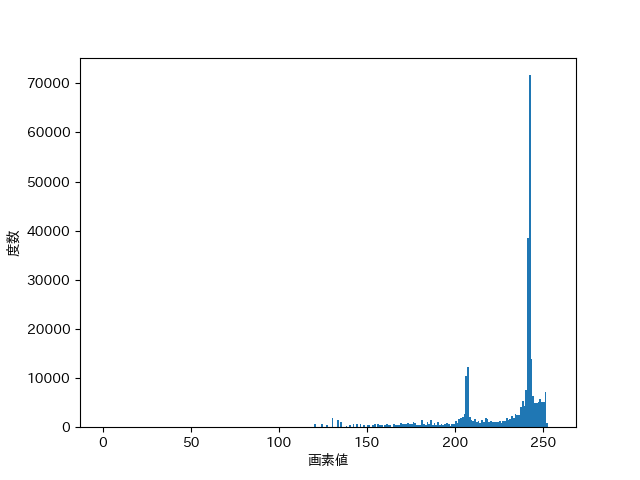
\includegraphics[width=\linewidth]{01_hist/gamma_defa_hist.png}
        \caption{図\ref{fig:gamma_defa}の濃淡ヒストグラム}
        \label{fig:gamma_defa_hist}
      \end{minipage}
      \vspace{0.5cm}
      \par
    % 下段
      \begin{minipage}{0.45\textwidth}
        \centering 
        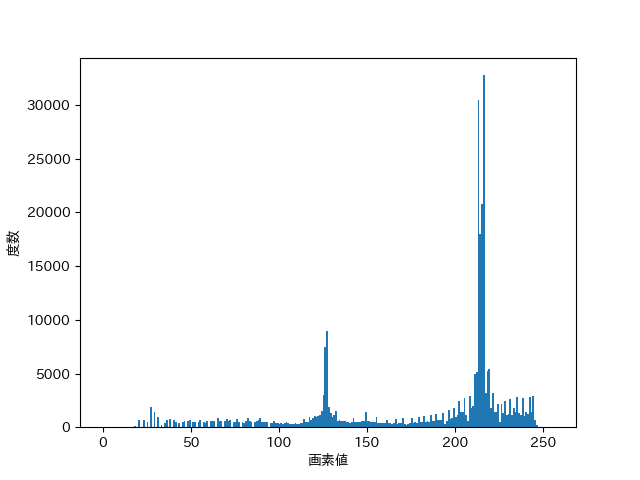
\includegraphics[width=\linewidth]{01_hist/gamma_hi_hist.png}
        \caption{図\ref{fig:gamma_hi}の濃淡ヒストグラム} 
        \label{fig:gamma_hi_hist}
      \end{minipage}%
      \hfill
      \begin{minipage}{0.45\textwidth}
        \centering
        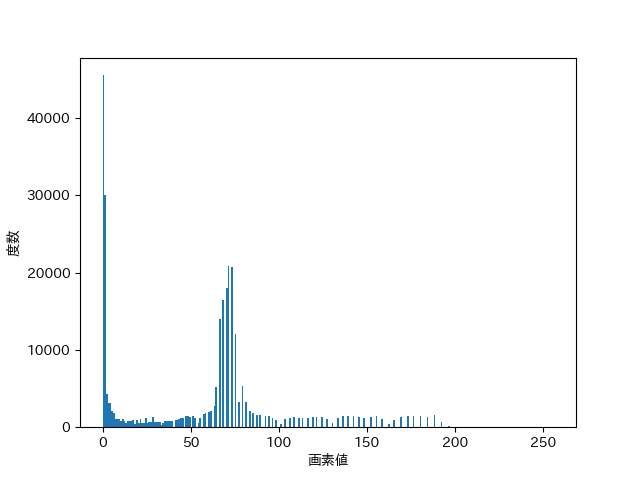
\includegraphics[width=\linewidth]{01_hist/gamma_low_hist.png}
        \caption{図\ref{fig:gamma_low}の濃淡ヒストグラム}
        \label{fig:gamma_low_hist}
      \end{minipage}
     \end{figure}

   \subsection{考察}
   線形変換ではコントラストが低い図\ref{fig:woman-g2}に対して，変換後の範囲を(0,255)とした図\ref{fig:sen_defa}は明暗がはっきりとしたコントラストの高い画像となっている．
   元画像のヒストグラム(図\ref{fig:woman-g2_hist})と変換後のヒストグラム(図\ref{fig:sen_defa_hist})を比較しても，画素値が全体に広く分布していることがわかる．一方，範囲を(100,255)とした場合は，
   画素値の下限が100に制限されるため，図\ref{fig:sen_hi}では本来黒くなるべき箇所が明るいグレーに変換され，全体的に白っぽく霞んだ画像となっている．
   図\ref{fig:sen_hi_hist}のヒストグラムにおいても暗い部分(0～99)の画素が存在せず，200～250付近に画素が集中していることがわかる．また，範囲を(0,150)とした場合は，
   画素値の上限が150に制限されるため，図\ref{fig:sen_low}では本来白くなるべき箇所が暗いグレーに抑え込まれ，全体的に暗く沈んだ画像となっている．
   図\ref{fig:sen_low_hist}のヒストグラムにおいても，明るい部分(151～255)の画素が存在せず，100～150付近に画素が集中していることがわかる．
   これらの結果から，線形変換においては指定する最大値と最小値の差が広がるほどコントラストが向上し，差が狭まるほどコントラストが低下することが確認できた．

   ガンマ補正では，標準的な濃淡を持つ図\ref{fig:woman-g}に対して，$\gamma$=5.0とした場合，図\ref{fig:gamma_defa}から，画像全体が白飛びしたような非常に明るい画像となっていることがわかる．
   図\ref{fig:gamma_defa_hist}でも，ヒストグラムが右側に大きく偏っていることがわかる．同様に$\gamma$=1.5とした場合も図\ref{fig:gamma_hi_hist}より，ヒストグラムが右に偏っていることが分かるが，図\ref{fig:gamma_hi}では図\ref{fig:woman-g}に比べて
   適度に明るくなった自然な結果が得られている．一方$\gamma=0.2$のように$\gamma<1$に設定した場合は，図\ref{fig:gamma_low_hist}よりヒストグラムが左側に偏り，図\ref{fig:gamma_low}のように画像全体が暗く沈み込んだ結果となることがわかる．
   これらの結果から，ガンマ補正は$\gamma>1$で画像が明るく，$\gamma<1$で画像が暗くなり，線形変換のように全体を均等に変化させるのではなく，特定の明るさに調整できる処理であることが確認できた．
  \section{課題2}
   \subsection{実験内容}
    平滑化について，プログラムのkernelの値を変更すると図\ref{fig:woman-g}がどの様に変化するか確認する．
    また，ノイズを付与された画像(図\ref{fig:woman-goma}と図\ref{fig:woman_spike})からノイズを除去するには，どのフィルタを使うと効果的であるか，理由とともに考察する．
    \begin{figure}[H]
      \centering
      \begin{minipage}{0.45\textwidth}
        \centering
        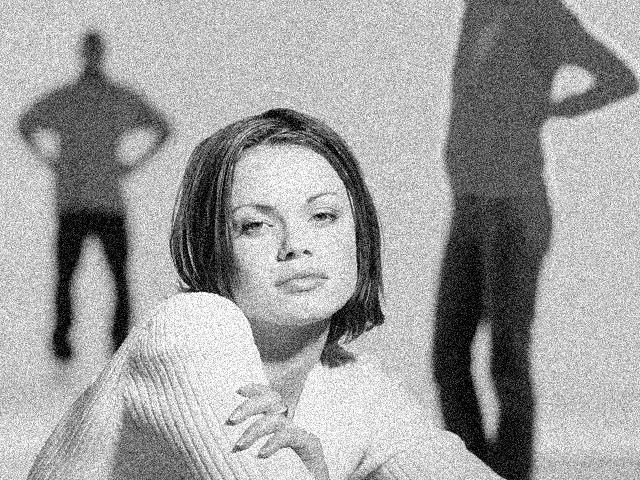
\includegraphics[width=\linewidth]{02_image/woman-goma.jpg}
        \caption{ごま塩ノイズ画像}
        \label{fig:woman-goma}
      \end{minipage}
      \hfill
      \begin{minipage}{0.45\textwidth}
        \centering
        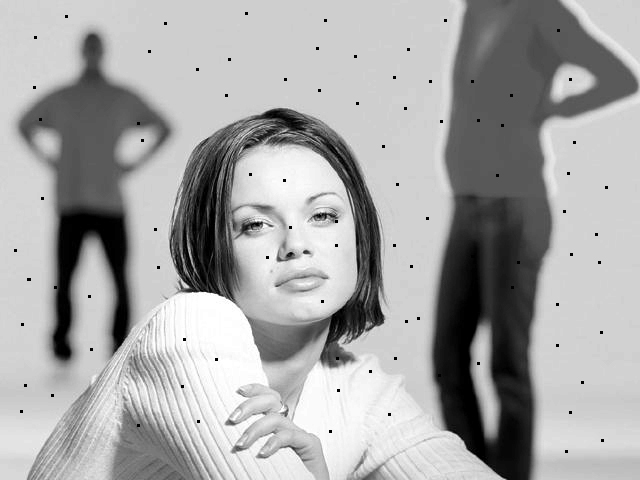
\includegraphics[width=\linewidth]{02_image/woman-spike.jpg}
        \caption{スパイクノイズ画像}
        \label{fig:woman_spike}
      \end{minipage}
    \end{figure}
   \subsection{平滑化の結果}
    平滑化において最も自然で高い効果が得られるガウシアンフィルタで図\ref{fig:woman-g}に対してのカーネルサイズ(ksize)の変更による平滑化の強さの変化を比較する．ksizeを(3,3)とした際の画像を図\ref{fig:gausu_low}に，(5,5)とした際の画像を図\ref{fig:gausu_medi}に，(11,11)とした際の画像を図\ref{fig:gausu_hi}に示す．
         \begin{figure}[H]
      \centering
      % 上段
      \begin{minipage}{0.45\textwidth}
        \centering
        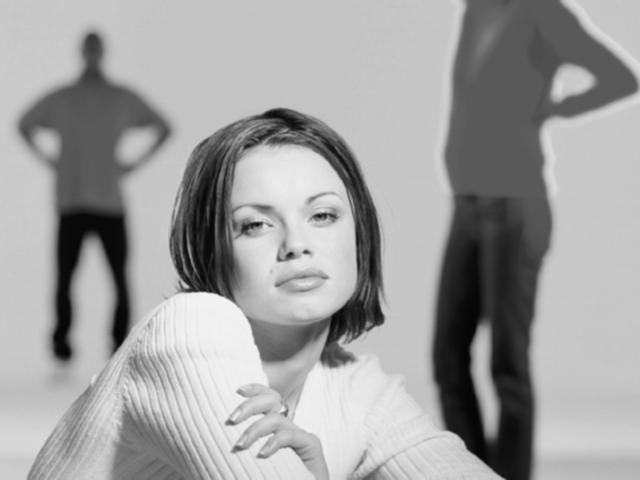
\includegraphics[width=\linewidth]{02_image/gaussian_low.jpg}
        \caption{ksize=(3,3)でのガウシアンフィルタ後の画像}
        \label{fig:gausu_low}
      \end{minipage}
      \hfill
      \begin{minipage}{0.45\textwidth}
        \centering
        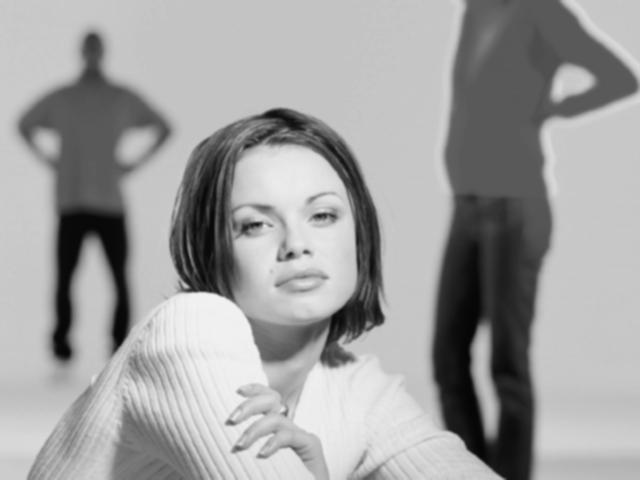
\includegraphics[width=\linewidth]{02_image/gaussian_median.jpg}
        \caption{ksize=(5,5)でのガウシアンフィルタ後の画像}
        \label{fig:gausu_medi}
      \end{minipage}
      \vspace{0.5cm}
      \par
    % 下段
      \begin{minipage}{0.45\textwidth}
        \centering 
        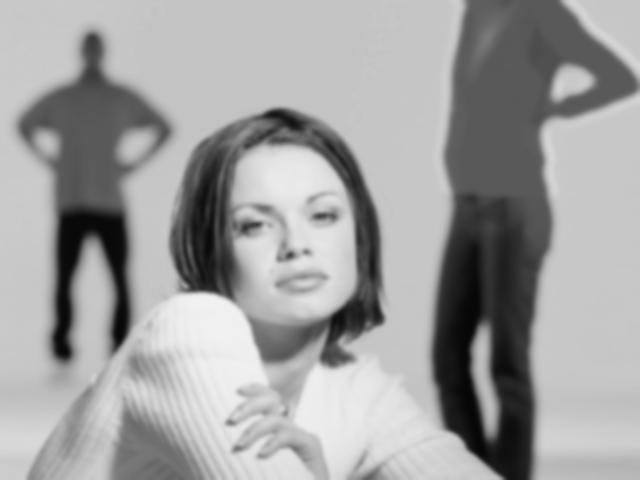
\includegraphics[width=\linewidth]{02_image/gaussian_hi.jpg}
        \caption{ksize=(11,11)でのガウシアンフィルタ後の画像}  
        \label{fig:gausu_hi} 
      \end{minipage}
      \hfill
      \begin{minipage}{0.45\textwidth}
      \end{minipage}
    \end{figure}

\subsection{ノイズ除去の結果}
カーネルサイズをksize=5に統一した状態で，ごま塩ノイズ画像(図\ref{fig:woman-goma})とスパイクノイズ画像(図\ref{fig:woman_spike})に対して各平滑化フィルタを適用し，ノイズ除去効果を比較した．それぞれの処理結果は以下のとおりである．
\begin{itemize}
 \item 移動平均フィルタ：ごま塩ノイズへの適用結果を図\ref{fig:movemean_goma}に，スパイクノイズへの適用結果を図\ref{fig:movemean_spike}に示す．
 \item ガウシアンフィルタ：ごま塩ノイズへの適用結果を図\ref{fig:gaussian_goma}に，スパイクノイズへの適用結果を図\ref{fig:gaussian_spike}に示す．
 \item メディアンフィルタ：ごま塩ノイズへの適用結果を図\ref{fig:medianfilter_goma}に，スパイクノイズへの適用結果を図\ref{fig:medianfilter_spike}に示す．
\end{itemize}

\begin{figure}[H]
  \centering
  \begin{minipage}{0.45\textwidth}
    \centering
    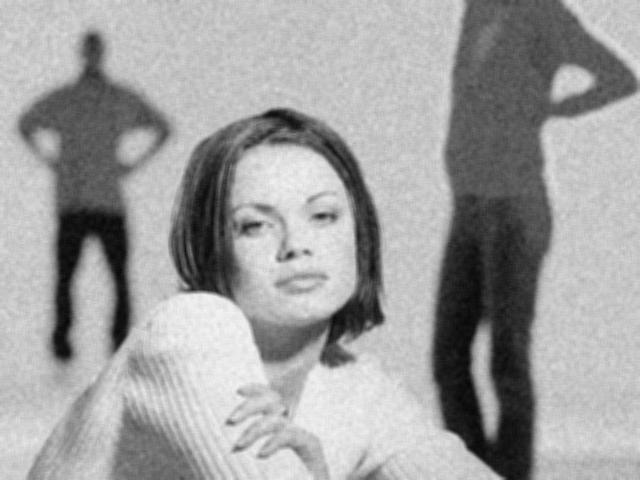
\includegraphics[width=\linewidth]{02_image/movemean_goma.jpg}
    \caption{図\ref{fig:woman-goma}に移動平均フィルタを適用した画像}
    \label{fig:movemean_goma}
  \end{minipage}
  \hfill
  \begin{minipage}{0.45\textwidth}
    \centering
    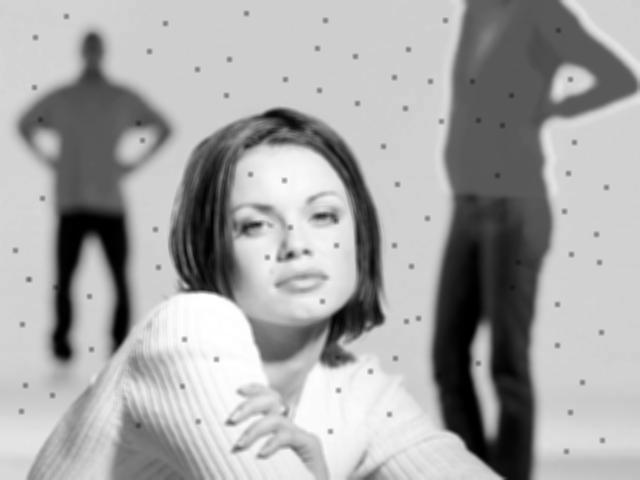
\includegraphics[width=\linewidth]{02_image/movemean_spike.jpg}
    \caption{図\ref{fig:woman_spike}に移動平均フィルタを適用した画像}
    \label{fig:movemean_spike}
  \end{minipage}
  
  \vspace{0.6cm} % 行間の余白
  \par
  \begin{minipage}{0.45\textwidth}
    \centering
    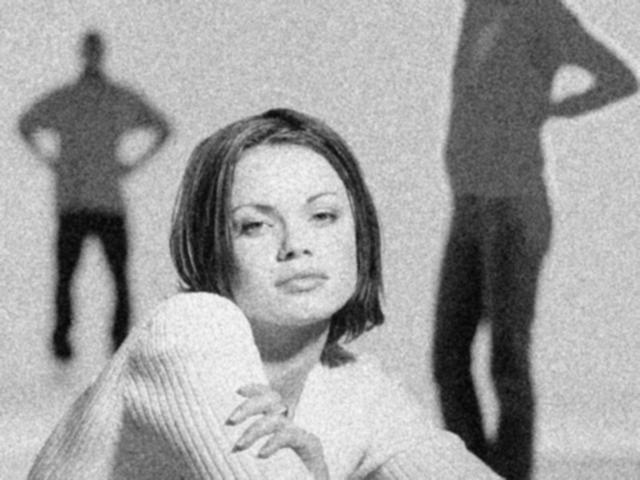
\includegraphics[width=\linewidth]{02_image/gaussian_goma.jpg}
    \caption{図\ref{fig:woman-goma}にガウシアンフィルタを適用した画像}
    \label{fig:gaussian_goma}
  \end{minipage}
  \hfill
  \begin{minipage}{0.45\textwidth}
    \centering
    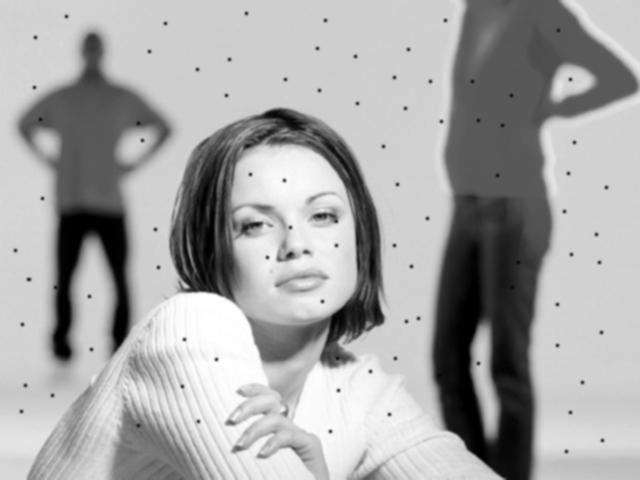
\includegraphics[width=\linewidth]{02_image/gaussian_spike.jpg}
    \caption{図\ref{fig:woman_spike}にガウシアンフィルタを適用した画像}
    \label{fig:gaussian_spike}
  \end{minipage}
  
  \vspace{0.6cm} % 行間の余白
  \par
  \begin{minipage}{0.45\textwidth}
    \centering
    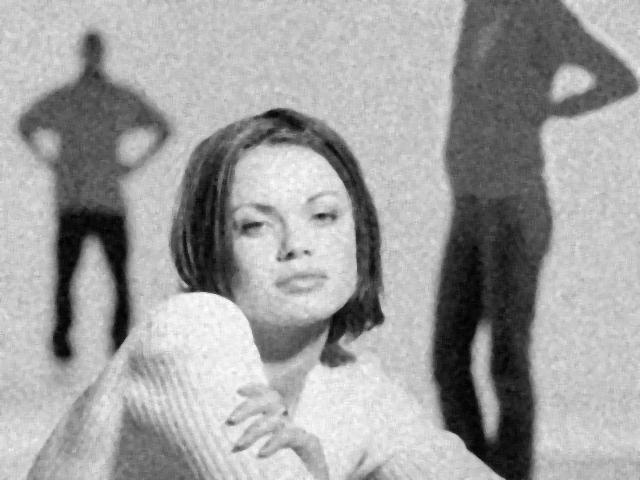
\includegraphics[width=\linewidth]{02_image/medianfilter_goma.jpg}
    \caption{図\ref{fig:woman-goma}にメディアンフィルタを適用した画像}
    \label{fig:medianfilter_goma}
  \end{minipage}
  \hfill
  \begin{minipage}{0.45\textwidth}
    \centering
    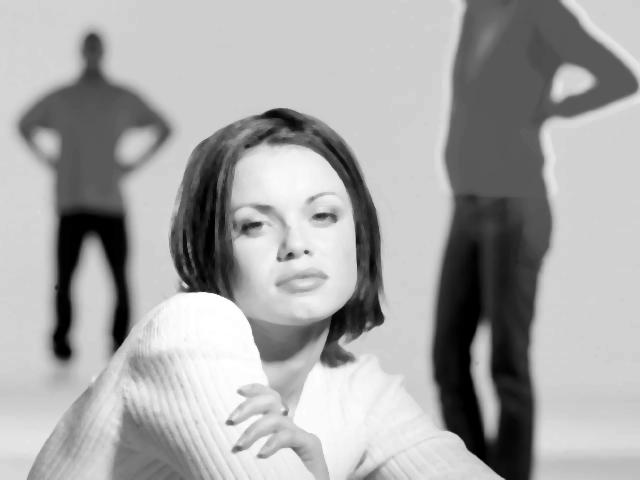
\includegraphics[width=\linewidth]{02_image/medianfilter_spike.jpg}
    \caption{図\ref{fig:woman_spike}にメディアンフィルタを適用した画像}
    \label{fig:medianfilter_spike}
  \end{minipage}

\end{figure}
  \subsection{考察}
   図\ref{fig:gausu_low}では，平滑化の範囲が狭く，背景の人物の輪郭等の細部の情報がはっきりとわかる．図\ref{fig:gausu_medi}では，図\ref{fig:gausu_low}と比較すると，少しぼやけてきており，主要な輪郭は残っているが細部の情報は失われ始めている．
   図\ref{fig:gausu_hi}では，平滑化の影響が最も表れており，細部の情報はぼやけてしまい，ほとんどわからなくなってしまっている．
   これらの結果から，カーネルサイズの拡大は平滑化を強める一方で，画像本来の鮮明さを失わせることが確認できた．

   次に、ごま塩ノイズの画像(図\ref{fig:woman-goma})および，スパイクノイズの画像(図\ref{fig:woman_spike})に対して各平滑化フィルタを適用した結果を比較する．
   移動平均フィルタ(図\ref{fig:movemean_goma}，\ref{fig:movemean_spike})とガウシアンフィルタ(図\ref{fig:gaussian_goma}，\ref{fig:gaussian_spike})では，どちらのノイズも周囲ににじんで残ってしまっていることが確認できる．これは，これらのフィルタが周囲の画素
   の平均を取る性質があるため，極端なノイズの値も計算に混ざってしまったためと考えられる．一方で，メディアンフィルタ(図\ref{fig:medianfilter_goma}，\ref{fig:medianfilter_spike})では、スパイクノイズを除去できているとは言えないが他フィルタに比べて背景や女性の顔に注目した際にもっともノイズが少なく，ツルッとした表面になっていることが確認できる．
   一方で，スパイクフィルタについては完全にノイズを除去出来ていることが確認できる．これは，メディアンフィルタが値を並び替えて中央値を取る性質があるため，ノイズのような極端な値が計算から除外されたためと考えられる．
   これらの結果から，突発的な点ノイズの除去にはメディアンフィルタが最も適していることが確認できた．
\end{document}